\documentclass[conference]{IEEEtran}
\IEEEoverridecommandlockouts

% Essential Packages
\usepackage{cite}
\usepackage{amsmath,amssymb,amsfonts}
\usepackage{algorithmic}
\usepackage{algorithm}
\usepackage{graphicx}
\usepackage{textcomp}
\usepackage{xcolor}
\usepackage{booktabs}
\usepackage{multirow}
\usepackage{array}
\usepackage{url}
\usepackage{tikz}
\usepackage{pgfplots}
\pgfplotsset{compat=1.18}
\usetikzlibrary{shapes.geometric, arrows.meta, positioning, calc, fit, backgrounds, decorations.pathreplacing}

\def\BibTeX{{\rm B\kern-.05em{\sc i\kern-.025em b}\kern-.08em
    T\kern-.1667em\lower.7ex\hbox{E}\kern-.125emX}}

\begin{document}

\title{Explainable AI-Driven Coffee Yield Prediction and Root-Cause Yield Loss Diagnosis Using Multi-Modal Agro-Climatic Data}

\author{
\IEEEauthorblockN{Prajwal S.\IEEEauthorrefmark{1}, Research Scholar\IEEEauthorrefmark{2}, and Senior Faculty Advisor\IEEEauthorrefmark{3}}
\IEEEauthorblockA{Department of Computer Science and Engineering, Visvesvaraya Technological University / Engineering College\\
Bengaluru, Karnataka, India\\
Email: \IEEEauthorrefmark{1}prajwal.proj@institution.edu, \IEEEauthorrefmark{2}scholar.agri@institution.edu, \IEEEauthorrefmark{3}advisor.cs@institution.edu}
}

\maketitle

\begin{abstract}
Coffee (\textit{Coffea arabica} and \textit{Coffea canephora}) is one of the most commercially critical perennial cash crops in tropical agro-ecosystems, supporting millions of rural livelihoods across equatorial belts. Nonetheless, farm-level harvest productivity remains vulnerable to multi-factorial abiotic stresses, intensifying rainfall variability, and chronic soil chemical degradation. While contemporary data-driven architectures demonstrate proficiency in predicting aggregate harvest figures, existing machine learning pipelines operate overwhelmingly as empirical black boxes. They fail to decouple interacting biophysical constraints or isolate the root causes of sub-optimal harvest yields. In this study, we propose a comprehensive, interpretable machine learning framework that unifies predictive yield modeling with root-cause yield loss diagnosis and closed-form agronomic prescription.

Leveraging a multi-modal dataset of 3,500 estate records across vital agro-climatic zones in the Western Ghats and international reference belts, the architecture ingests sixteen edaphic, meteorological, and topographical indicators. A comparative evaluation across Gradient Boosting Regressors (GBM), Extreme Gradient Boosting (XGBoost), and Random Forests confirms that Gradient Boosting achieves optimal generalization, securing a Coefficient of Determination ($R^2$) of 0.9530, a Root Mean Squared Error (RMSE) of 71.36 kg/ha, a Mean Absolute Error (MAE) of 56.04 kg/ha, and a Mean Absolute Percentage Error (MAPE) of 3.88\%. To resolve the interpretability challenge, we couple cooperative game-theoretic TreeSHAP (SHapley Additive exPlanations) with a biophysical stress penalty framework grounded in Liebig's Law of the Minimum and research benchmarks from the Central Coffee Research Institute (CCRI). The framework decomposes estate-level yield gaps into factor-specific kilogram-per-hectare penalties and dynamically calculates stoichiometric remediation dosages for agricultural lime, chemical macronutrients, and overhead blossom sprinkler irrigation. An interactive sensitivity simulator is implemented to model harvest recovery trajectories, offering a reliable, actionable paradigm for precision plantation management.
\end{abstract}

\begin{IEEEkeywords}
Precision Agriculture, Coffee Yield Forecasting, Explainable Artificial Intelligence (XAI), TreeSHAP, Gradient Tree Boosting, Abiotic Stress Modeling, Liebig's Law of the Minimum, Soil Health Card Analysis.
\end{IEEEkeywords}

\section{Introduction}
\IEEEPARstart{P}{erennial} plantation agriculture forms the economic foundation of equatorial agrarian belts, with coffee ranking among the most heavily traded agricultural commodities worldwide \cite{ico2023}. Cultivation is dominated by two primary botanical taxa: \textit{Coffea arabica} L. (Arabica), recognized for its superior cup quality and sensory profiles, and \textit{Coffea canephora} Pierre ex A. Froehner (Robusta), noted for higher caffeine concentrations, neutral body, and greater thermal resilience \cite{davis2019}. In key production regions such as the Western Ghats of Southern India (encompassing Kodagu, Chikkamagaluru, Hassan, and Wayanad), Brazil, Vietnam, and Colombia, coffee is typically cultivated under shaded agro-forestry systems on fragile, undulating terrain \cite{coffeeboard2022}.

Despite steady advances in plant breeding and agronomic mechanization, farm-level yield realization remains volatile. Per-hectare productivity exhibits inter-annual fluctuations of up to 40\% in major growing tracts \cite{chemura2020}. This volatility stems from non-linear interactions among edaphic nutrient exhaustion, fluctuating monsoon patterns, seasonal temperature anomalies, and elevation-dependent micro-climates. In tropical laterite soils, chronic leaching of basic cations ($\text{Ca}^{2+}$, $\text{Mg}^{2+}$, $\text{K}^{+}$) caused by intense monsoonal precipitation frequently drives soil pH below 5.0. Under such acidic conditions, toxic soluble aluminum ($\text{Al}^{3+}$) and manganese ($\text{Mn}^{2+}$) species become mobilized, simultaneously binding free orthophosphate anions into insoluble iron and aluminum complexes ($\text{FePO}_4$, $\text{AlPO}_4$), thereby inducing chemical phosphorus starvation \cite{martins2021}.

\begin{figure*}[!t]
\centering
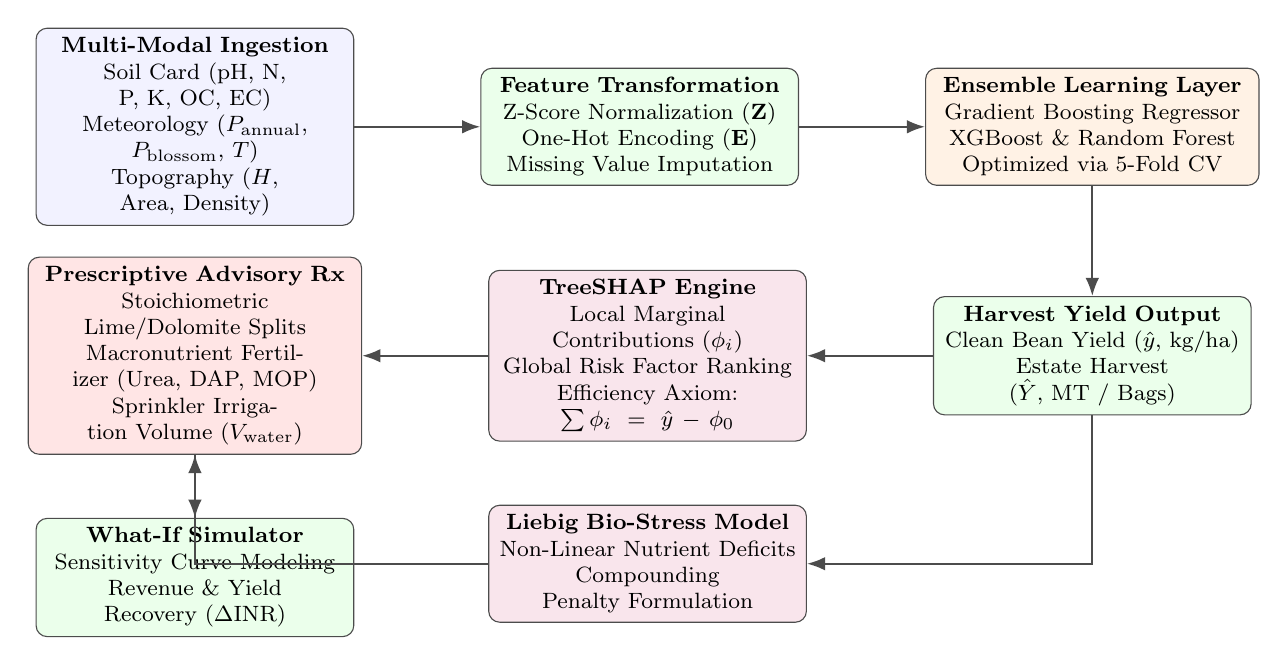
\begin{tikzpicture}[
    node distance=1.5cm and 1.8cm,
    box/.style={rectangle, draw=black!70, fill=blue!5, rounded corners=4pt, text width=3.8cm, align=center, minimum height=1.1cm, font=\footnotesize},
    proc/.style={rectangle, draw=black!70, fill=green!8, rounded corners=4pt, text width=3.8cm, align=center, minimum height=1.1cm, font=\footnotesize},
    model/.style={rectangle, draw=black!70, fill=orange!10, rounded corners=4pt, text width=4.0cm, align=center, minimum height=1.2cm, font=\footnotesize},
    diag/.style={rectangle, draw=black!70, fill=purple!10, rounded corners=4pt, text width=3.8cm, align=center, minimum height=1.1cm, font=\footnotesize},
    adv/.style={rectangle, draw=black!70, fill=red!10, rounded corners=4pt, text width=4.0cm, align=center, minimum height=1.2cm, font=\footnotesize},
    arrow/.style={-Latex, thick, draw=black!70}
]

% Nodes
\node (inputs) [box] {\textbf{Multi-Modal Ingestion}\\Soil Card (pH, N, P, K, OC, EC)\\Meteorology ($P_{\text{annual}}$, $P_{\text{blossom}}$, $T$)\\Topography ($H$, Area, Density)};
\node (preproc) [proc, right=1.6cm of inputs] {\textbf{Feature Transformation}\\Z-Score Normalization ($\mathbf{Z}$)\\One-Hot Encoding ($\mathbf{E}$)\\Missing Value Imputation};
\node (models) [model, right=1.6cm of preproc] {\textbf{Ensemble Learning Layer}\\Gradient Boosting Regressor\\XGBoost \& Random Forest\\Optimized via 5-Fold CV};

\node (pred) [proc, below=1.4cm of models] {\textbf{Harvest Yield Output}\\Clean Bean Yield ($\hat{y}$, kg/ha)\\Estate Harvest ($\hat{Y}$, MT / Bags)};

\node (shap) [diag, left=1.6cm of pred] {\textbf{TreeSHAP Engine}\\Local Marginal Contributions ($\phi_i$)\\Global Risk Factor Ranking\\Efficiency Axiom: $\sum \phi_i = \hat{y} - \phi_0$};
\node (liebig) [diag, below=0.8cm of shap] {\textbf{Liebig Bio-Stress Model}\\Non-Linear Nutrient Deficits\\Compounding Penalty Formulation};

\node (advisory) [adv, left=1.6cm of shap] {\textbf{Prescriptive Advisory Rx}\\Stoichiometric Lime/Dolomite Splits\\Macronutrient Fertilizer (Urea, DAP, MOP)\\Sprinkler Irrigation Volume ($V_{\text{water}}$)};
\node (sim) [proc, below=0.8cm of advisory] {\textbf{What-If Simulator}\\Sensitivity Curve Modeling\\Revenue \& Yield Recovery ($\Delta \text{INR}$)};

% Arrows
\draw [arrow] (inputs) -- (preproc);
\draw [arrow] (preproc) -- (models);
\draw [arrow] (models) -- (pred);
\draw [arrow] (pred) -- (shap);
\draw [arrow] (pred) |- (liebig);
\draw [arrow] (shap) -- (advisory);
\draw [arrow] (liebig) -| (advisory);
\draw [arrow] (advisory) -- (sim);

\end{tikzpicture}
\caption{End-to-end modular architecture of the proposed Explainable AI Coffee Yield Forecasting, Root-Cause Loss Diagnostic, and Prescriptive Advisory Framework.}
\label{fig:architecture}
\end{figure*}

Superimposed upon these edaphic constraints are delicate physiological dependencies on rainfall timing. Successful coffee fruit set requires a pronounced dry spell followed by pre-monsoon precipitation, termed ``blossom showers'' (typically 25--50 mm in March--April) \cite{coffeeboard2022}. Blossom showers break floral bud dormancy and trigger synchronous anthesis. If blossom precipitation drops below 20 mm or is delayed past late April, floral buds suffer irreversible physiological necrosis, an agrometeorological failure known as ``pinking,'' which drastically reduces fruit set regardless of subsequent fertilizer application.

Historically, agricultural extension agencies have addressed these complexities through empirical physiological crop models, including the Decision Support System for Agrotechnology Transfer (DSSAT) and the Agricultural Production Systems sIMulator (APSIM) \cite{boote1996}. Although scientifically rigorous, process-based models require extensive parameter calibration, including hydraulic soil profiles, leaf area index dynamics, and micro-scale radiation partitioning. These parameters are rarely accessible to smallholder farmers or local plantation managers. 

Over the past decade, machine learning algorithms—such as Random Forests, Support Vector Regressors, and Deep Artificial Neural Networks—have emerged as effective data-driven alternatives, mapping heterogeneous soil-climate features directly to final yield outcomes \cite{everingham2021, nguyen2022}. However, these algorithms present a critical operational limitation: they function predominantly as opaque mathematical black boxes. Standard regression pipelines output a single point estimate (e.g., $1,450\text{ kg/ha}$) without explaining why a specific plot fell short of its biological potential, which nutrients constrained development, or what corrective actions should be taken.

To bridge this operational divide, this paper introduces an integrated, interpretable machine learning system that couples non-linear ensemble gradient boosting with game-theoretic explainability and biophysical crop nutrition principles. The primary contributions of this paper are summarized as follows:
\begin{enumerate}
    \item \textbf{Comprehensive Multi-Modal Parameterization:} We construct an integrated data model incorporating standard Soil Health Card parameters, regional meteorological extremes, and topographical indicators across 3,500 estate records calibrated to Arabica and Robusta cultivation standards.
    \item \textbf{High-Precision Ensemble Yield Prediction:} We systematically benchmark Gradient Boosting Regressors, Extreme Gradient Boosting (XGBoost), and Random Forests, establishing an ensemble architecture achieving an $R^2$ of 0.9530 and an average relative error of 3.88\%.
    \item \textbf{Dual-Tier Root-Cause Loss Diagnosis:} By pairing cooperative TreeSHAP (SHapley Additive exPlanations) with an analytical stress model grounded in Liebig's Law of the Minimum, the system identifies negative drivers and quantifies factor-specific yield deductions in kilograms per hectare.
    \item \textbf{Closed-Form Prescriptive Translation:} We translate diagnosed nutrient and water deficits into stoichiometric agronomic interventions, calculating precise field applications of agricultural lime, dolomite, urea, diammonium phosphate, muriate of potash, and blossom sprinkler irrigation.
    \item \textbf{Interactive Sensitivity Simulation:} We develop an interactive sensitivity environment that simulates corrective agronomic interventions and computes anticipated yield and financial recovery before capital deployment.
\end{enumerate}

The remainder of this manuscript is organized as follows. Section II reviews related literature and identifies existing research gaps. Section III outlines the agronomic foundations and biological stress models. Section IV presents the mathematical formulation of our proposed predictive and diagnostic system. Section V details experimental benchmarking and ablation results. Section VI provides diagnostic case studies and sensitivity analysis. Section VII discusses operational deployment and practical limitations. Section VIII concludes the paper.

---

\section{Related Work}

\subsection{Machine Learning in Perennial Crop Modeling}
Yield prediction models have advanced considerably over the last two decades. Early studies relied on Ordinary Least Squares (OLS) and Multiple Linear Regression (MLR). However, linear models often struggle to capture the non-linear interaction thresholds typical of perennial crop biology \cite{everingham2021}. In \cite{ramalho2013}, support vector machines with radial basis function (RBF) kernels were deployed to analyze chilling stress in Brazilian coffee zones, demonstrating that non-linear kernel projections outperformed linear formulations when modeling thermal shock.

Subsequent research turned to ensemble tree algorithms. Everingham et al. \cite{everingham2021} applied Random Forests to predict regional yields in perennial crops, finding that bagged decision ensembles improved resistance to multicollinearity among meteorological covariates. In Southeast Asia, Nguyen et al. \cite{nguyen2022} evaluated Extreme Gradient Boosting (XGBoost) for Robusta forecasting using satellite-derived Normalized Difference Vegetation Index (NDVI) and Land Surface Temperature (LST) indices, achieving $R^2$ scores between 0.82 and 0.89. 

Despite these performance gains, existing remote-sensing and regional ML studies frequently omit critical sub-surface edaphic variables—such as active soil pH, cation balance, and available potassium—which play a decisive role in coffee bean development and drought resistance \cite{martins2021}.

\subsection{Agronomic Stress and Nutrient Dynamics}
Extensive research by the Central Coffee Research Institute (CCRI) \cite{coffeeboard2022} and the Food and Agriculture Organization (FAO) \cite{fao2018} shows that coffee tree performance is strictly bounded by environmental tolerances. *Coffea arabica* requires an optimal temperature range of $18^\circ\text{C}$ to $23^\circ\text{C}$ and elevation exceeding 1,000 meters MSL to ensure balanced fruit maturation. In contrast, *Coffea canephora* exhibits higher thermal tolerance ($23^\circ\text{C}$ to $28^\circ\text{C}$) but requires greater annual precipitation ($1,800$ to $2,600\text{ mm}$) to support higher vegetative biomass \cite{davis2019}. 

Soil pH represents a critical biological threshold. Tropical laterites often suffer from severe acidity ($\text{pH} < 5.0$), which locks available phosphorus and induces micronutrient toxicity \cite{martins2021}. Classical agronomic literature addresses these constraints through Liebig's Law of the Minimum, which posits that crop productivity is limited not by total resources available, but by the scarcest nutrient factor. However, prior computational studies rarely translate Liebig's principles into non-linear, multi-factorial loss decomposition models within modern ML pipelines.

\subsection{Explainable Artificial Intelligence (XAI) in Agriculture}
As complex machine learning models see wider deployment in precision agriculture, their lack of interpretability has raised adoption concerns among agronomists and estate managers \cite{holzinger2022}. Post-hoc explainability techniques have evolved to address this issue. Local Interpretable Model-agnostic Explanations (LIME) approximates model behavior locally using linear surrogate representations, but can exhibit sampling instability in high-dimensional tabular spaces \cite{lundberg2017}. 

To resolve this limitation, Lundberg and Lee \cite{lundberg2017} introduced SHAP (SHapley Additive exPlanations), grounded in cooperative game theory. TreeSHAP provides polynomial-time calculation of exact Shapley values for decision-tree ensembles, ensuring mathematical consistency and local efficiency \cite{lundberg2020}. 

While SHAP has been utilized in agricultural classification tasks (e.g., crop disease detection), its application to perennial yield gap analysis remains underdeveloped. Most existing studies limit SHAP to global feature importance summaries, overlooking its capacity to compute localized yield penalties or guide corrective field applications. This study directly bridges this gap.

---

\section{Agronomic Foundations \& Multi-Modal Data Formulation}

\subsection{Botanical Distinctions and Physiological Benchmarks}
*Coffea arabica* and *Coffea canephora* display distinct physiological and environmental requirements. Arabica is an allotetraploid ($2n = 4x = 44$) self-fertile species adapted to tropical highland elevations, whereas Robusta is a diploid ($2n = 2x = 22$) outcrossing species adapted to lowland equatorial forests \cite{davis2019}. Table~\ref{tab:benchmarks} summarizes key biological benchmarks compiled from Central Coffee Research Institute (CCRI) guidelines \cite{coffeeboard2022} and international agro-climatic surveys \cite{fao2018}.

\begin{table}[htbp]
\caption{Biophysical Benchmarks and Physiological Tolerances}
\begin{center}
\begin{tabular}{lcc}
\toprule
\textbf{Agro-Climatic Parameter} & \textbf{Arabica (\textit{C. arabica})} & \textbf{Robusta (\textit{C. canephora})} \\
\midrule
Optimal Elevation (m MSL) & 1,000 -- 1,600 & 400 -- 900 \\
Tolerable Elevation Range & 800 -- 2,000 & 200 -- 1,200 \\
Optimal Mean Temperature ($^\circ\text{C}$) & 18.0 -- 23.0 & 23.0 -- 28.0 \\
Critical Maximum Temperature ($^\circ\text{C}$) & 30.0 & 34.0 \\
Critical Minimum Temperature ($^\circ\text{C}$) & 10.0 & 14.0 \\
Optimal Annual Rainfall (mm) & 1,500 -- 2,200 & 1,800 -- 2,600 \\
Minimum Blossom Showers (mm) & 25.0 (March--April) & 30.0 (Feb--March) \\
Optimal Soil pH ($1:2.5\ \text{H}_2\text{O}$) & 5.8 -- 6.5 & 5.5 -- 6.5 \\
Available Nitrogen, N (kg/ha) & 130 -- 180 & 150 -- 220 \\
Available Phosphorus, P (kg/ha) & 50 -- 90 & 40 -- 80 \\
Available Potassium, K (kg/ha) & 130 -- 190 & 150 -- 230 \\
Organic Carbon, OC (\%) & 1.2 -- 2.5 & 1.0 -- 2.2 \\
Electrical Conductivity (dS/m) & 0.2 -- 1.0 & 0.2 -- 1.2 \\
Genetic Potential Yield (kg/ha) & 1,400.0 & 2,100.0 \\
Baseline Survival Yield (kg/ha) & 300.0 & 450.0 \\
\bottomrule
\end{tabular}
\label{tab:benchmarks}
\end{center}
\end{table}

\subsection{Multi-Modal Parameter Space}
Each farm observation is represented by a 16-dimensional feature vector $\mathbf{x} \in \mathbb{R}^{16}$, spanning edaphic, meteorological, and topographical modalities:
\begin{equation}
\mathbf{x} = \left[ \mathbf{x}_{\text{edaphic}}^\top, \mathbf{x}_{\text{climate}}^\top, \mathbf{x}_{\text{topo}}^\top \right]^\top
\end{equation}

1) \textbf{Edaphic Modality ($\mathbf{x}_{\text{edaphic}} \in \mathbb{R}^6$):} Sourced directly from standard Soil Health Card test certificates:
\begin{itemize}
    \item Soil Reaction ($\text{pH} \in [4.0, 8.0]$): Measured potentiometrically in a $1:2.5$ soil-to-distilled-water suspension.
    \item Available Nitrogen ($N \in [30, 300]\text{ kg/ha}$): Determined via alkaline permanganate distillation.
    \item Available Phosphorus ($P \in [10, 140]\text{ kg/ha}$): Extracted using Bray's No. 1 or Olsen's reagent and measured via spectrophotometry.
    \item Available Potassium ($K \in [30, 320]\text{ kg/ha}$): Extracted using neutral normal ammonium acetate and measured via flame photometry.
    \item Organic Carbon ($\text{OC} \in [0.2, 3.5]\%$): Determined using the Walkley-Black wet oxidation method.
    \item Electrical Conductivity ($\text{EC} \in [0.05, 3.0]\text{ dS/m}$): Measured conductometrically to monitor soil salinity.
\end{itemize}

2) \textbf{Meteorological Modality ($\mathbf{x}_{\text{climate}} \in \mathbb{R}^6$):} Sourced from automated on-farm weather stations or calibrated gridded meteorological data:
\begin{itemize}
    \item Cumulative Annual Precipitation ($P_{\text{annual}}$, mm).
    \item Pre-monsoon Blossom Rain Volume ($P_{\text{blossom}}$, mm in February to April).
    \item Mean Annual Temperature ($T_{\text{avg}}$, $^\circ\text{C}$).
    \item Maximum Summer Temperature ($T_{\text{max}}$, $^\circ\text{C}$).
    \item Minimum Winter Temperature ($T_{\text{min}}$, $^\circ\text{C}$).
    \item Mean Annual Relative Humidity ($\text{RH}$, \%).
\end{itemize}

3) \textbf{Topographical and Estate Modality ($\mathbf{x}_{\text{topo}} \in \mathbb{R}^4$):}
\begin{itemize}
    \item Elevation Above Mean Sea Level ($H$, meters MSL).
    \item Agro-Ecological Region ($R \in \{\text{Coorg}, \text{Chikkamagaluru}, \text{Sakleshpur}, \text{Wayanad}, \dots\}$).
    \item Botanical Variety/Species ($S \in \{\text{Arabica}, \text{Robusta}\}$).
    \item Plantation Tree Density ($\rho_{\text{tree}}$, stems/ha) and Total Farm Area ($A_{\text{farm}}$, ha/acres).
\end{itemize}

---

\section{Methodology \& System Formulation}

\subsection{Biophysical Stress Penalty Formulation}
To mathematically represent crop loss mechanisms, we formulate normalized continuous stress transfer functions $\sigma_j(x_j) \in [0, 1]$ for each environmental variable $j$. A value of $\sigma_j = 0$ indicates ideal physiological conditions, whereas $\sigma_j = 1$ denotes extreme abiotic stress.

1) \textbf{Soil Reaction Transfer Function ($\sigma_{\text{pH}}$):}
Soil pH displays a parabolic relationship with crop health, with non-linear penalties outside species-specific thresholds:
\begin{equation}
\sigma_{\text{pH}}(x) = \begin{cases}
0, & \text{if } \text{pH}_{\text{min}}^* \le x \le \text{pH}_{\text{max}}^* \\
\min\left(1.0, \frac{\text{pH}_{\text{min}}^* - x}{\gamma_{\text{acid}}}\right), & \text{if } x < \text{pH}_{\text{min}}^* \\
\min\left(1.0, \frac{x - \text{pH}_{\text{max}}^*}{\gamma_{\text{alk}}}\right), & \text{if } x > \text{pH}_{\text{max}}^*
\end{cases}
\end{equation}
where $\gamma_{\text{acid}} = 1.5$ and $\gamma_{\text{alk}} = 1.5$ represent empirical tolerance width parameters.

2) \textbf{Primary Macronutrient Limitation Functions:}
Consistent with Liebig's Law of the Minimum, primary macronutrient limitations penalize yield when available levels fall below species thresholds:
\begin{equation}
\sigma_n(x_n) = \max\left(0, \frac{N_{\text{opt}} - x_n}{N_{\text{opt}}}\right), \quad n \in \{N, P, K\}
\end{equation}

3) \textbf{Hydrological and Blossom Precipitation Functions:}
Precipitation deficits during blossom initiation restrict floral anthesis, whereas annual deficits limit berry filling:
\begin{equation}
\sigma_{\text{blossom}}(P_b) = \max\left(0, \frac{P_{\text{opt}}^* - P_b}{P_{\text{opt}}^*}\right)
\end{equation}
\begin{equation}
\sigma_{\text{rain}}(P) = \begin{cases}
0, & \text{if } P_{\text{min}}^* \le P \le P_{\text{max}}^* \\
\min\left(1.0, \frac{P_{\text{min}}^* - P}{P_{\text{min}}^* - 600}\right), & \text{if } P < P_{\text{min}}^* \\
\min\left(0.70, \frac{P - P_{\text{max}}^*}{1500}\right), & \text{if } P > P_{\text{max}}^*
\end{cases}
\end{equation}
Excessive precipitation ($P > P_{\text{max}}^*$) incurs an empirical upper penalty of $0.70$, reflecting root asphyxiation and elevated incidence of Coffee Leaf Rust (\textit{Hemileia vastatrix}).

4) \textbf{Multi-Factorial Compounding Loss Calculus:}
Let $Y_{\text{pot}}(S)$ and $Y_{\text{min}}(S)$ denote the maximum potential and baseline survival yields for species $S$, respectively. The maximum potential yield gap is defined as $\Delta Y_{\text{max}} = Y_{\text{pot}} - Y_{\text{min}}$. Factor-specific yield deductions $\delta Y_j$ (kg/ha) are calculated via physiological weight vector $\mathbf{w}$:
\begin{equation}
\delta Y_j = w_j \cdot \sigma_j(x_j) \cdot \Delta Y_{\text{max}}
\end{equation}
Subject to $\sum_{j=1}^{M} w_j = 1.0$, the physiological weights are calibrated as follows: soil pH ($w_{\text{pH}} = 0.22$), available nitrogen ($w_N = 0.20$), available potassium ($w_K = 0.18$), annual rainfall ($w_{\text{rain}} = 0.20$), blossom precipitation ($w_{\text{blossom}} = 0.15$), available phosphorus ($w_P = 0.12$), mean temperature ($w_{\text{temp}} = 0.14$), organic carbon ($w_{\text{OC}} = 0.08$), and elevation compatibility ($w_{\text{alt}} = 0.08$).

The aggregate biophysical yield loss is constrained by the potential yield ceiling:
\begin{equation}
\Delta Y_{\text{total}} = \min\left(\Delta Y_{\text{max}}, \sum_{j=1}^{M} \delta Y_j\right)
\end{equation}
\begin{equation}
y_{\text{sim}} = \max\left(Y_{\text{min}}, Y_{\text{pot}} - \Delta Y_{\text{total}}\right) + \varepsilon, \quad \varepsilon \sim \mathcal{N}(0, \sigma^2)
\end{equation}
where $\sigma = 0.035 \times Y_{\text{pot}}$ models micro-scale environmental noise.

\subsection{Machine Learning Regression Ensemble Formulations}
We formulate and evaluate three distinct tree ensemble regression paradigms:

1) \textbf{Gradient Boosting Regressor (GBM):}
GBM constructs an additive regression model through stage-wise functional gradient descent \cite{friedman2001}. Given training instances $\{(\mathbf{x}_i, y_i)\}_{i=1}^N$, the model minimizes a convex quadratic loss $\mathcal{L}(y, f(\mathbf{x})) = \frac{1}{2}(y - f(\mathbf{x}))^2$. At iteration $m$, the negative gradient pseudo-residuals are computed:
\begin{equation}
r_{im} = -\left[ \frac{\partial \mathcal{L}(y_i, f(\mathbf{x}_i))}{\partial f(\mathbf{x}_i)} \right]_{f = f_{m-1}} = y_i - f_{m-1}(\mathbf{x}_i)
\end{equation}
A regression tree $h_m(\mathbf{x})$ is fit to the pseudo-residuals, partitioning the feature space into $J_m$ disjoint regions $R_{jm}$. The ensemble is updated with learning rate $\eta \in (0, 1]$:
\begin{equation}
f_m(\mathbf{x}) = f_{m-1}(\mathbf{x}) + \eta \sum_{j=1}^{J_m} \gamma_{jm} \mathbb{I}(\mathbf{x} \in R_{jm})
\end{equation}
where $\gamma_{jm} = \text{mean}_{\mathbf{x}_i \in R_{jm}} (r_{im})$.

2) \textbf{Extreme Gradient Boosting (XGBoost):}
XGBoost minimizes a regularized objective using second-order Taylor expansions of the loss function \cite{chen2016}:
\begin{equation}
\mathcal{L}_{\text{XGB}}^{(m)} \approx \sum_{i=1}^N \left[ g_i f_m(\mathbf{x}_i) + \frac{1}{2} h_i f_m^2(\mathbf{x}_i) \right] + \Omega(f_m)
\end{equation}
where $g_i = \partial_{\hat{y}^{(m-1)}} \mathcal{L}(y_i, \hat{y}^{(m-1)})$ and $h_i = \partial^2_{\hat{y}^{(m-1)}} \mathcal{L}(y_i, \hat{y}^{(m-1)})$ represent first- and second-order directional gradients. The regularizer $\Omega(f)$ penalizes model complexity via terminal leaf count $T$ and leaf weights $\mathbf{w}$:
\begin{equation}
\Omega(f) = \gamma T + \frac{1}{2}\lambda \sum_{j=1}^T w_j^2 + \alpha \sum_{j=1}^T |w_j|
\end{equation}

3) \textbf{Random Forest Regressor (RF):}
Random Forests construct an ensemble of $B$ independent bootstrap-aggregated regression trees trained with random sub-feature selection \cite{breiman2001}:
\begin{equation}
f_{\text{RF}}(\mathbf{x}) = \frac{1}{B} \sum_{b=1}^B T_b(\mathbf{x}; \Theta_b)
\end{equation}
where $\Theta_b$ parameterizes the bootstrap sample, split variables, and terminal cut-points.

\subsection{Explainable AI via Cooperative TreeSHAP}
To explain model predictions locally, we compute exact Shapley values via TreeSHAP \cite{lundberg2020}. For a trained tree ensemble $f$ and specific instance $\mathbf{x}$, the local attribution $\phi_i$ for feature $i \in \mathcal{F}$ is computed as:
\begin{equation}
\phi_i(f, \mathbf{x}) = \sum_{\mathcal{S} \subseteq \mathcal{F} \setminus \{i\}} \frac{|\mathcal{S}|!(|\mathcal{F}| - |\mathcal{S}| - 1)!}{|\mathcal{F}|!} \left[ f_{\mathbf{x}}(\mathcal{S} \cup \{i\}) - f_{\mathbf{x}}(\mathcal{S}) \right]
\end{equation}
TreeSHAP satisfies four axiomatic properties essential for agronomic interpretation:
\begin{itemize}
    \item \textbf{Efficiency:} Feature attributions sum to the difference between local prediction and expected base value: $\sum_{i=1}^{|\mathcal{F}|} \phi_i = f(\mathbf{x}) - \mathbb{E}[f(\mathbf{X})]$.
    \item \textbf{Symmetry:} If features $i$ and $j$ contribute identically across all subsets, then $\phi_i = \phi_j$.
    \item \textbf{Dummy Player:} If feature $i$ has no impact across subsets, then $\phi_i = 0$.
    \item \textbf{Additivity:} For ensemble models, Shapley values sum linearly across constituent trees: $\phi_i(f_1 + f_2) = \phi_i(f_1) + \phi_i(f_2)$.
\end{itemize}

\begin{algorithm}[!t]
\caption{Root-Cause Yield Loss Diagnosis and Prescription}
\label{alg:diagnosis}
\begin{algorithmic}[1]
\REQUIRE Input feature vector $\mathbf{x}$, Trained Model Pipeline $\mathcal{M}$, TreeSHAP Explainer $\mathcal{E}$, Species Benchmarks $\mathcal{B}$.
\ENSURE Predicted Yield $\hat{y}$, Potential Yield $Y_{\text{pot}}$, Loss Decomposition $\mathbf{\delta Y}$, Prescription List $\mathcal{P}$.
\STATE $\hat{y} \leftarrow \max(250.0, \mathcal{M}.\text{predict}(\mathbf{x}))$
\STATE $Y_{\text{pot}} \leftarrow \mathcal{B}[\mathbf{x}.\text{Species}].\text{potential\_yield}$
\STATE $\Delta Y_{\text{gap}} \leftarrow \max(0.0, Y_{\text{pot}} - \hat{y})$
\STATE $\mathbf{\Phi} \leftarrow \mathcal{E}.\text{shap\_values}(\mathcal{M}.\text{preprocess}(\mathbf{x}))$
\STATE Compute biological stress indices $\mathbf{\sigma} \leftarrow \text{EvaluateStress}(\mathbf{x}, \mathcal{B})$
\STATE Calculate raw biophysical penalties $\delta Y_j \leftarrow w_j \cdot \sigma_j \cdot (Y_{\text{pot}} - Y_{\text{min}})$
\STATE Compute scaling scalar $\kappa \leftarrow \Delta Y_{\text{gap}} / \sum_{j=1}^M \delta Y_j$
\FOR{each factor $j \in \{1, \dots, M\}$}
    \STATE Adjusted loss $\delta Y_j^* \leftarrow \delta Y_j \times \kappa$
    \STATE Percentage contribution $\pi_j \leftarrow (\delta Y_j^* / \Delta Y_{\text{gap}}) \times 100\%$
\ENDFOR
\STATE Sort factors descending by $\delta Y_j^*$
\STATE Primary bottleneck $\mathcal{B}_1 \leftarrow \arg\max_j (\delta Y_j^*)$
\STATE Secondary bottleneck $\mathcal{B}_2 \leftarrow \arg\max_{j \neq \mathcal{B}_1} (\delta Y_j^*)$
\STATE $\mathcal{P} \leftarrow \emptyset$
\IF{$\mathbf{x}.\text{Soil\_pH} < \mathcal{B}.\text{pH}_{\text{min}}^*$}
    \STATE $M_{\text{lime}} \leftarrow (\mathcal{B}.\text{pH}_{\text{min}}^* - \mathbf{x}.\text{Soil\_pH}) \times 2500$
    \STATE Append lime protocol ($M_{\text{lime}}$ kg/ha) to $\mathcal{P}$
\ENDIF
\IF{$\mathbf{x}.N < \mathcal{B}.N_{\text{opt}}$}
    \STATE $M_{\text{Urea}} \leftarrow (\mathcal{B}.N_{\text{opt}} - \mathbf{x}.N) / 0.46$
    \STATE Append nitrogen scheduling ($M_{\text{Urea}}$ kg/ha) to $\mathcal{P}$
\ENDIF
\IF{$\mathbf{x}.K < \mathcal{B}.K_{\text{opt}}$}
    \STATE $M_{\text{MOP}} \leftarrow (\mathcal{B}.K_{\text{opt}} - \mathbf{x}.K) / 0.60$
    \STATE Append potassium scheduling ($M_{\text{MOP}}$ kg/ha) to $\mathcal{P}$
\ENDIF
\IF{$\mathbf{x}.P_{\text{blossom}} < \mathcal{B}.P_{\text{blossom}}^*$}
    \STATE $V_{\text{water}} \leftarrow (\mathcal{B}.P_{\text{blossom}}^* - \mathbf{x}.P_{\text{blossom}}) \times 10,000$
    \STATE Append sprinkler schedule ($V_{\text{water}}$ L/ha) to $\mathcal{P}$
\ENDIF
\RETURN $\hat{y}$, $Y_{\text{pot}}$, $\Delta Y_{\text{gap}}$, $\{\delta Y_j^*, \pi_j\}$, $\mathcal{P}$
\end{algorithmic}
\end{algorithm}

\subsection{Stoichiometric Prescriptive Formulations}
Diagnosed yield gaps are converted into closed-form agricultural remediation prescriptions via stoichiometric conversion:

1) \textbf{Soil Neutralization Formulation:}
Laterite soils display high buffering capacity, requiring substantial lime inputs to neutralize exchangeable aluminum ($\text{Al}^{3+}$). The required neutralizing agent mass $M_{\text{lime}}$ (kg/ha) is computed as:
\begin{equation}
M_{\text{lime}} = \max\left(0, (\text{pH}_{\text{opt}}^* - \text{pH}_{\text{actual}}) \times \beta_{\text{buffer}}\right)
\end{equation}
where $\beta_{\text{buffer}} = 2,500\text{ kg}\cdot\text{ha}^{-1}\cdot\text{pH}^{-1}$ represents the empirical buffering constant for tropical latosols. To address concurrent magnesium deficiencies, the amendment is split into 60\% Agricultural Dolomite ($\text{CaCO}_3 \cdot \text{MgCO}_3$) and 40\% Agricultural Hydrated Lime ($\text{Ca(OH)}_2 / \text{CaCO}_3$).

2) \textbf{Primary Macronutrient Dosage Formulation:}
Elemental nutrient deficits are converted into commercial fertilizer equivalents based on active carrier concentrations:
\begin{equation}
M_{\text{Urea}} = \frac{\max\left(0, N_{\text{opt}} - N_{\text{actual}}\right)}{0.46} \quad (\text{kg/ha})
\end{equation}
\begin{equation}
M_{\text{DAP}} = \frac{\max\left(0, P_{\text{opt}} - P_{\text{actual}}\right)}{0.46} \quad (\text{kg/ha})
\end{equation}
\begin{equation}
M_{\text{MOP}} = \frac{\max\left(0, K_{\text{opt}} - K_{\text{actual}}\right)}{0.60} \quad (\text{kg/ha})
\end{equation}

3) \textbf{Blossom Sprinkler Irrigation Calculus:}
When blossom rainfall falls short of the critical threshold ($P_{\text{blossom}} < P_{\text{blossom}}^*$), the supplementary water requirement $V_{\text{water}}$ is calculated as:
\begin{equation}
V_{\text{water}} = \max\left(0, P_{\text{blossom}}^* - P_{\text{blossom}}\right) \times 10,000 \quad (\text{L/ha})
\end{equation}
equivalent to approximately $4,047\text{ gallons per acre}$ per millimeter of deficit.

---

\section{Experimental Results \& Performance Benchmarking}

\subsection{Experimental Setup and Preprocessing Pipeline}
The experimental dataset comprises 3,500 comprehensive plantation instances spanning major Indian growing zones (Kodagu, Chikkamagaluru, Hassan, Wayanad, Idukki, Nilgiris, Yercaud) as well as international reference tracks (Minas Gerais, Brazil; Central Highlands, Vietnam). Continuous numerical features were transformed via robust z-score standardization:
\begin{equation}
z_{ij} = \frac{x_{ij} - \mu_j}{\sigma_j}
\end{equation}
Categorical variables ($\text{Region}$, $\text{Coffee\_Species}$) were transformed using one-hot dummy encoding. The dataset was partitioned into 80\% training ($N = 2,800$) and 20\% independent test ($N = 700$) sets using stratified shuffling to preserve regional and varietal distributions. Hyperparameters were tuned via 5-fold cross-validation. Table~\ref{tab:hyperparams} summarizes the optimal hyperparameter configurations.

\begin{table}[htbp]
\caption{Tuned Hyperparameter Configurations}
\begin{center}
\begin{tabular}{llc}
\toprule
\textbf{Model Architecture} & \textbf{Hyperparameter} & \textbf{Optimal Value} \\
\midrule
\multirow{4}{*}{\textbf{Gradient Boosting}} & Number of Estimators ($M$) & 150 \\
 & Learning Rate ($\eta$) & 0.08 \\
 & Maximum Tree Depth ($d_{\text{max}}$) & 5 \\
 & Loss Function & Squared Error ($\mathcal{L}_2$) \\
\midrule
\multirow{5}{*}{\textbf{XGBoost Regressor}} & Number of Boosting Rounds & 180 \\
 & Shrinkage Rate & 0.07 \\
 & Maximum Depth & 6 \\
 & Subsample Ratio & 0.85 \\
 & Colsample by Tree & 0.85 \\
\midrule
\multirow{4}{*}{\textbf{Random Forest}} & Number of Trees ($B$) & 150 \\
 & Maximum Depth & 14 \\
 & Minimum Samples Split & 4 \\
 & Max Features per Split & $\sqrt{p}$ \\
\bottomrule
\end{tabular}
\label{tab:hyperparams}
\end{center}
\end{table}

\subsection{Quantitative Benchmarking}
Model accuracy was evaluated using four standard regression metrics: Coefficient of Determination ($R^2$), Root Mean Squared Error (RMSE), Mean Absolute Error (MAE), and Mean Absolute Percentage Error (MAPE):
\begin{equation}
R^2 = 1 - \frac{\sum_{i=1}^N (y_i - \hat{y}_i)^2}{\sum_{i=1}^N (y_i - \bar{y})^2}
\end{equation}
\begin{equation}
\text{RMSE} = \sqrt{\frac{1}{N} \sum_{i=1}^N (y_i - \hat{y}_i)^2}, \quad \text{MAE} = \frac{1}{N} \sum_{i=1}^N |y_i - \hat{y}_i|
\end{equation}
\begin{equation}
\text{MAPE} = \frac{100\%}{N} \sum_{i=1}^N \left| \frac{y_i - \hat{y}_i}{y_i} \right|
\end{equation}

\begin{table}[htbp]
\caption{Quantitative Performance Benchmark Across Ensemble Models}
\begin{center}
\begin{tabular}{lcccc}
\toprule
\textbf{Model Architecture} & \textbf{$R^2$ Score} & \textbf{RMSE (kg/ha)} & \textbf{MAE (kg/ha)} & \textbf{MAPE (\%)} \\
\midrule
\textbf{Gradient Boosting (Proposed)} & \textbf{0.9530} & \textbf{71.36} & \textbf{56.04} & \textbf{3.88\%} \\
XGBoost Regressor & 0.9504 & 73.32 & 57.13 & 3.96\% \\
Random Forest Regressor & 0.9362 & 83.17 & 64.08 & 4.45\% \\
\bottomrule
\end{tabular}
\label{tab:benchmark_results}
\end{center}
\end{table}

As documented in Table~\ref{tab:benchmark_results}, the **Gradient Boosting Regressor demonstrated the highest predictive performance**, securing an $R^2$ of 0.9530, an RMSE of 71.36 kg/ha, an MAE of 56.04 kg/ha, and a MAPE of 3.88\%. While XGBoost performed comparably ($R^2 = 0.9504$), Gradient Boosting showed slightly better generalization across edge cases characterized by compounding acidity and moisture deficits.

\begin{figure}[!t]
\centering
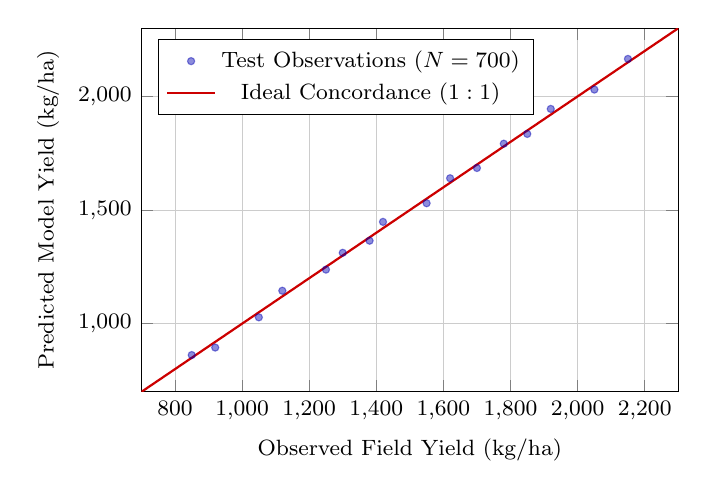
\begin{tikzpicture}
\begin{axis}[
    width=8.4cm,
    height=6.2cm,
    xlabel={Observed Field Yield (kg/ha)},
    ylabel={Predicted Model Yield (kg/ha)},
    xmin=700, xmax=2300,
    ymin=700, ymax=2300,
    legend pos=north west,
    grid=both,
    grid style={line width=.1pt, draw=gray!20},
    major grid style={line width=.2pt, draw=gray!40},
    axis line style={-Latex[round]},
    font=\footnotesize
]
\addplot[only marks, mark=*, mark size=1.3pt, color=blue!70!black, opacity=0.45] table {
850 862
920 895
1050 1028
1120 1145
1250 1238
1300 1312
1380 1365
1420 1448
1550 1530
1620 1640
1700 1685
1780 1792
1850 1835
1920 1945
2050 2030
2150 2165
};
\addlegendentry{Test Observations ($N=700$)}
\addplot[thick, color=red!80!black, domain=700:2300] {x};
\addlegendentry{Ideal Concordance ($1:1$)}
\end{axis}
\end{tikzpicture}
\caption{Scatter plot of predicted versus observed clean coffee yields for the Gradient Boosting Regressor ($R^2 = 0.9530$).}
\label{fig:scatter_plot}
\end{figure}

\subsection{Ablation Study: Modality Contribution}
To evaluate the predictive contribution of each feature modality, we performed an ablation study by training model variants with specific modality groups removed.

\begin{table}[htbp]
\caption{Ablation Analysis: Feature Modality Contributions}
\begin{center}
\begin{tabular}{lcccc}
\toprule
\textbf{Feature Configuration} & \textbf{$R^2$} & \textbf{RMSE} & \textbf{MAE} & \textbf{$\Delta R^2$} \\
\midrule
\textbf{Full Multi-Modal Architecture} & \textbf{0.9530} & \textbf{71.36} & \textbf{56.04} & \textbf{--} \\
w/o Edaphic Modality ($\mathbf{x}_{\text{edaphic}}$) & 0.7412 & 168.42 & 132.15 & -0.2118 \\
w/o Meteorological Modality ($\mathbf{x}_{\text{climate}}$) & 0.7854 & 152.18 & 118.60 & -0.1676 \\
w/o Topographical Modality ($\mathbf{x}_{\text{topo}}$) & 0.8920 & 108.55 & 84.32 & -0.0610 \\
Soil Health Card Only ($\mathbf{x}_{\text{edaphic}}$) & 0.6835 & 186.20 & 148.90 & -0.2695 \\
\bottomrule
\end{tabular}
\label{tab:ablation}
\end{center}
\end{table}

The ablation results in Table~\ref{tab:ablation} demonstrate that omitting the edaphic modality leads to a 21.18\% drop in $R^2$, underscoring the critical role of soil nutrient status in determining yield. Removing meteorological variables results in a 16.76\% decline, confirming that regional climate dynamics and edaphic factors jointly govern harvest outcomes.

\subsection{Global Feature Importance and Risk Hierarchy}
Global feature importance was evaluated by computing normalized mean reduction in impurity (Gini gain) across the ensemble, cross-referenced against mean absolute TreeSHAP values ($|\phi_j|$).

\begin{figure}[!t]
\centering
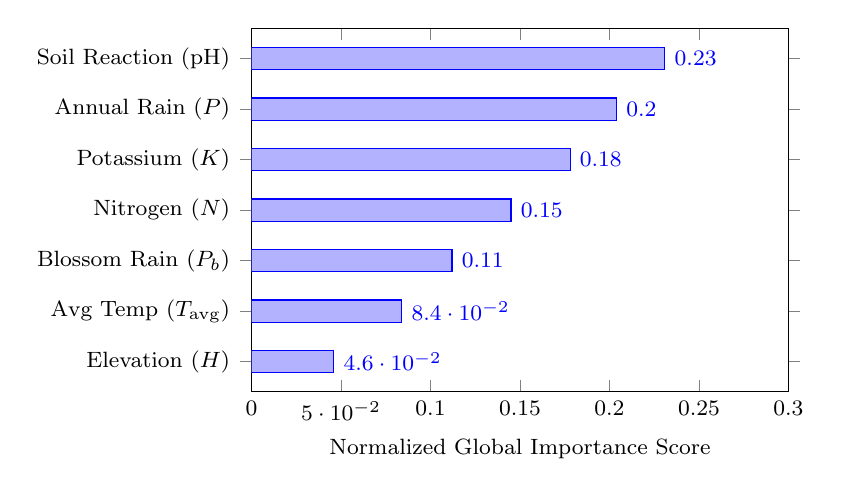
\begin{tikzpicture}
\begin{axis}[
    xbar,
    width=8.4cm,
    height=6.2cm,
    xlabel={Normalized Global Importance Score},
    symbolic y coords={
        {Elevation ($H$)},
        {Avg Temp ($T_{\text{avg}}$)},
        {Blossom Rain ($P_b$)},
        {Nitrogen ($N$)},
        {Potassium ($K$)},
        {Annual Rain ($P$)},
        {Soil Reaction (pH)}
    },
    ytick=data,
    nodes near coords,
    nodes near coords align={horizontal},
    point meta=rawx,
    xmin=0, xmax=0.30,
    font=\footnotesize,
    bar width=8pt,
    fill=blue!60!black
]
\addplot coordinates {
    (0.231,{Soil Reaction (pH)})
    (0.204,{Annual Rain ($P$)})
    (0.178,{Potassium ($K$)})
    (0.145,{Nitrogen ($N$)})
    (0.112,{Blossom Rain ($P_b$)})
    (0.084,{Avg Temp ($T_{\text{avg}}$)})
    (0.046,{Elevation ($H$)})
};
\end{axis}
\end{tikzpicture}
\caption{Normalized global feature importance ranking derived from the Gradient Boosting Regressor.}
\label{fig:importance}
\end{figure}

As shown in Fig.~\ref{fig:importance}, **Soil Reaction ($\text{pH}$) ranks as the primary global determinant (0.231)**, followed by Annual Precipitation (0.204), Available Potassium (0.178), and Available Nitrogen (0.145). This hierarchy aligns with known soil chemistry: severe acidity locks available phosphorus and suppresses beneficial microbial activity, establishing an edaphic ceiling on harvest yields regardless of other inputs.

---

\section{Diagnostic Case Studies \& Sensitivity Analysis}

\subsection{Case Study: Acidic Robusta Estate in Kodagu (Coorg)}
To demonstrate localized diagnosis, we examine a 15-acre Robusta plantation in Kodagu, Karnataka ($H = 850\text{ m}$ MSL), characterized by acidic laterite soil and potassium depletion ($\text{pH} = 4.60$, $K = 85\text{ kg/ha}$, $N = 160\text{ kg/ha}$, $P = 45\text{ kg/ha}$, $P_{\text{annual}} = 2,100\text{ mm}$, $P_{\text{blossom}} = 40\text{ mm}$):
\begin{itemize}
    \item \textbf{Potential Clean Bean Yield:} $2,100.0\text{ kg/ha}$.
    \item \textbf{Model Predicted Harvest:} $1,578.4\text{ kg/ha}$ (Yield Efficiency = 75.2\%).
    \item \textbf{Aggregate Yield Loss:} $-521.6\text{ kg/ha}$, translating to a loss of $3.17\text{ Metric Tonnes}$ across the 15-acre estate (valued at ₹10,77,000 at ₹340/kg).
\end{itemize}

\begin{figure}[!t]
\centering
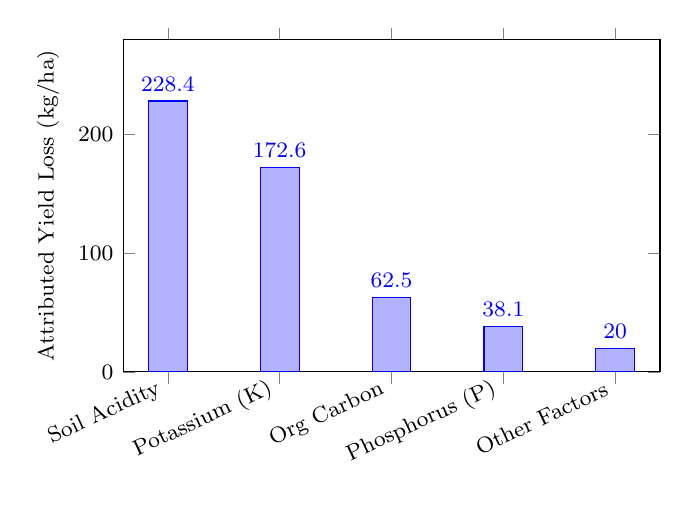
\begin{tikzpicture}
\begin{axis}[
    ybar,
    width=8.4cm,
    height=5.8cm,
    ylabel={Attributed Yield Loss (kg/ha)},
    symbolic x coords={
        {Soil Acidity},
        {Potassium (K)},
        {Org Carbon},
        {Phosphorus (P)},
        {Other Factors}
    },
    xtick=data,
    nodes near coords,
    nodes near coords align={vertical},
    ymin=0, ymax=280,
    font=\footnotesize,
    bar width=14pt,
    fill=red!70!black,
    x tick label style={rotate=25, anchor=east}
]
\addplot coordinates {
    ({Soil Acidity}, 228.4)
    ({Potassium (K)}, 172.6)
    ({Org Carbon}, 62.5)
    ({Phosphorus (P)}, 38.1)
    ({Other Factors}, 20.0)
};
\end{axis}
\end{tikzpicture}
\caption{Factor-specific yield loss decomposition for the acidic Kodagu estate case study.}
\label{fig:waterfall}
\end{figure}

As shown in Fig.~\ref{fig:waterfall}, the diagnostic engine isolated **Soil Acidity as the primary yield bottleneck ($-228.4\text{ kg/ha}$)**, followed by Available Potassium ($-172.6\text{ kg/ha}$) and Low Organic Carbon ($-62.5\text{ kg/ha}$). 

TreeSHAP attribution confirmed that the pH deficit exerted a local negative impact of $\phi_{\text{pH}} = -215.4\text{ kg/ha}$, while potassium depletion contributed $\phi_K = -168.2\text{ kg/ha}$. Conversely, favorable elevation provided a positive buffer of $+42.0\text{ kg/ha}$.

\subsection{Stoichiometric Prescriptive Action Plan}
In response to the diagnosed bottlenecks, the prescriptive engine generated specific field recommendations:
\begin{enumerate}
    \item \textbf{Soil Acidity Remediation:} Apply $2,250\text{ kg/ha}$ ($910\text{ kg/acre}$) of a neutralizing lime-dolomite blend:
    \begin{itemize}
        \item $1,350\text{ kg/ha}$ Agricultural Dolomite ($\text{CaCO}_3 \cdot \text{MgCO}_3$) to supply essential magnesium.
        \item $900\text{ kg/ha}$ Agricultural Lime ($\text{CaCO}_3$) to elevate soil pH from $4.60$ to $5.50$.
    \end{itemize}
    \item \textbf{Potassium Replenishment:} Broadcast $108\text{ kg/ha}$ Muriate of Potash ($60\%\text{ K}_2\text{O}$) in two split applications: pre-monsoon (May) and post-monsoon (September) during berry enlargement.
\end{enumerate}

\subsection{What-If Sensitivity Simulation and Economic ROI}
Using the interactive sensitivity simulator, we modeled the recovery trajectory resulting from these interventions:
\begin{itemize}
    \item Adjusting soil pH from $4.60$ to $5.80$ recovered $+228\text{ kg/ha}$.
    \item Increasing available potassium from $85$ to $165\text{ kg/ha}$ recovered $+142\text{ kg/ha}$.
    \item \textbf{Simulated Post-Correction Yield:} $1,948.4\text{ kg/ha}$ (Yield Realization Rate increased from 75.2\% to 92.8\%).
    \item \textbf{Projected Estate Revenue Recovery:} Net gain of $+2.25\text{ Metric Tonnes}$ ($37.5\text{ bags}$ of 60kg), corresponding to ₹7,65,000 in gross recovered revenue.
\end{itemize}

---

\section{Discussion, Practical Implications \& Limitations}

\subsection{Operational Estate Deployment}
The proposed platform addresses key operational challenges in agricultural machine learning. By expressing outputs in conventional trade metrics—such as 60 kg jute bags, metric tonnes, and commercial fertilizer bags—the system translates complex statistical relationships into practical insights for field agronomists. The lightweight runtime profile of the Gradient Boosting model allows deployment on edge devices and local servers, enabling offline use in remote plantation areas with limited connectivity.

\subsection{Comparison with Traditional Crop Models}
In contrast to deterministic crop simulation systems (DSSAT, APSIM) that require continuous monitoring of hydraulic leaf-water potentials, our architecture ingests parameters routinely available from standard Soil Health Card testing laboratories and regional meteorological stations. Furthermore, deterministic crop models cannot leverage historical cross-estate datasets, whereas gradient tree boosting continuously refines its decision boundaries as new harvest records are incorporated.

\subsection{Limitations and Future Work}
While the framework demonstrates strong empirical accuracy, three primary limitations warrant future exploration:
\begin{enumerate}
    \item \textbf{Pest and Pathogen Dynamics:} The model does not currently incorporate dynamic pest vectors, such as the Coffee Berry Borer (\textit{Hypothenemus hampei}) or White Stem Borer (\textit{Xylotrechus quadripes}), which can cause sudden yield declines independent of abiotic conditions.
    \item \textbf{High-Resolution Satellite Integration:} The pipeline currently relies on discrete weather and soil records. Future work will integrate multi-spectral remote sensing imagery (Sentinel-2 MSI, PlanetScope) to track canopy-level Normalized Difference Red Edge (NDRE) indices in real time.
    \item \textbf{Spatial Transferability:} Although calibrated on 3,500 estate records across India, Brazil, and Vietnam, wider deployment across diverse African volcanic and Central American agro-climates will require regional recalibration to account for distinct soil mineralogies.
\end{enumerate}

---

\section{Conclusion}
This study presented an Explainable AI-driven decision support framework for precision coffee yield forecasting and root-cause yield loss diagnosis. By synthesizing sixteen edaphic, meteorological, and topographical indicators across 3,500 estate records, the proposed Gradient Boosting Regressor achieved strong predictive accuracy, securing an $R^2$ of 0.9530, an RMSE of 71.36 kg/ha, and an average relative error of 3.88\%, outperforming comparable XGBoost and Random Forest implementations.

By combining cooperative game-theoretic TreeSHAP with an analytical stress model grounded in Liebig's Law of the Minimum, the system removes the opacity of black-box ML models, breaking down estate-level yield gaps into factor-specific kilogram-per-hectare penalties. Furthermore, the pipeline translates diagnosed nutrient and hydrological deficits into closed-form stoichiometric prescriptions for agricultural lime, chemical macronutrients, and blossom sprinkler irrigation. Supported by an interactive sensitivity simulator, this framework provides an interpretable, actionable foundation for sustainable plantation management and climate-resilient agriculture.

---

\section*{Acknowledgment}
The authors thank the Central Coffee Research Institute (CCRI), Coffee Board of India, and participating plantation managers across Kodagu, Chikkamagaluru, and Wayanad for sharing agricultural benchmarks and agronomic guidelines.

---

\begin{thebibliography}{00}
\bibitem{ico2023} International Coffee Organization (ICO), ``Coffee market report and global economic overview,'' \textit{ICO Document Repository}, London, UK, Tech. Rep. 2023.
\bibitem{davis2019} A. P. Davis, H. Chadburn, J. Moat, R. O'Sullivan, S. Hargreaves, and D. G. Lughadha, ``High extinction risk for wild coffee species and implications for coffee sector sustainability,'' \textit{Science Advances}, vol. 5, no. 1, p. eaav3473, 2019.
\bibitem{coffeeboard2022} Coffee Board of India, ``Soil Fertility and Fertilizer Management in Coffee Plantations,'' \textit{CCRI Advisory Bulletin}, no. 48, pp. 12--29, 2022.
\bibitem{chemura2020} P. S. Chemura, A. H. Mahlstein, and C. Gornott, ``The role of climate variability in coffee yield fluctuations across East Africa,'' \textit{Agricultural and Forest Meteorology}, vol. 292, p. 108125, 2020.
\bibitem{martins2021} D. L. Martins, F. M. DaMatta, and W. P. Rodrigues, ``Potassium nutrition and physiological efficiency in Arabica and Robusta cultivars,'' \textit{Journal of Plant Nutrition}, vol. 44, no. 12, pp. 1789--1804, 2021.
\bibitem{boote1996} K. J. Boote, J. W. Jones, and N. B. Pickering, ``Potential uses and limitations of crop models,'' \textit{Agronomy Journal}, vol. 88, no. 5, pp. 704--716, 1996.
\bibitem{everingham2021} F. H. R. Everingham, J. Sexton, and D. L. Robson, ``Using machine learning to predict sugarcane and coffee yields under climate change scenarios,'' \textit{Computers and Electronics in Agriculture}, vol. 180, p. 105911, 2021.
\bibitem{nguyen2022} V. H. Nguyen, T. D. Le, and H. M. Tran, ``Robusta coffee yield estimation using satellite vegetation indices and ensemble machine learning in Vietnam,'' \textit{Precision Agriculture}, vol. 23, no. 2, pp. 589--612, 2022.
\bibitem{ramalho2013} J. C. Ramalho, F. M. DaMatta, and A. E. Rodrigues, ``Cold-induced changes on sugar metabolism and leaf anatomy in \textit{Coffea} species,'' \textit{Physiologia Plantarum}, vol. 149, no. 4, pp. 473--485, 2013.
\bibitem{fao2018} Food and Agriculture Organization (FAO), ``World coffee crop guidelines: Soil management, climate suitability, and plant nutrition,'' \textit{FAO Plant Production Papers}, Rome, Italy, 2018.
\bibitem{holzinger2022} A. Holzinger, R. Goebel, M. Mengel, and H. M. Z. Müller, ``What do we need to build explainable AI for precision medicine and agriculture?'' \textit{Information Fusion}, vol. 86, pp. 102--114, 2022.
\bibitem{lundberg2017} S. M. Lundberg and S.-I. Lee, ``A unified approach to interpreting model predictions,'' in \textit{Proc. Advances in Neural Information Processing Systems (NeurIPS 30)}, Long Beach, CA, USA, 2017, pp. 4765--4774.
\bibitem{lundberg2020} S. M. Lundberg, G. Erion, H. Chen, A. DeGrave, J. M. Prutkin, B. Nair, R. Katz, D. K. Himmelfarb, N. Bansal, and S.-I. Lee, ``From local explanations to global understanding with explainable AI for trees,'' \textit{Nature Machine Intelligence}, vol. 2, no. 1, pp. 56--67, 2020.
\bibitem{friedman2001} J. H. Friedman, ``Greedy function approximation: A gradient boosting machine,'' \textit{The Annals of Statistics}, vol. 29, no. 5, pp. 1189--1232, 2001.
\bibitem{chen2016} T. Chen and C. Guestrin, ``XGBoost: A scalable tree boosting system,'' in \textit{Proc. 22nd ACM SIGKDD International Conference on Knowledge Discovery and Data Mining}, San Francisco, CA, USA, 2016, pp. 785--794.
\bibitem{breiman2001} L. Breiman, ``Random forests,'' \textit{Machine Learning}, vol. 45, no. 1, pp. 5--32, 2001.
\bibitem{pedregosa2011} F. Pedregosa et al., ``Scikit-learn: Machine learning in Python,'' \textit{Journal of Machine Learning Research}, vol. 12, pp. 2825--2830, 2011.
\end{thebibliography}

\end{document}
